\section{background}

In the Function-as-a-Service(FaaS)\cite{berkeley-view} incarnation of the serverless model,
the smallest unit of calculation used is a serverless function written by the user.
When the serverless computing platform receives a service request or a predefined event is triggered,
the serverless computing platform will initialize a temporary execution sandbox(containers\cite{container-in-serverless-1,container-in-serverless-2} or virtual machines\cite{firecracker,vm-in-serverless-1}, etc.),
and run the function uploaded by the user in the sandbox to process the request. After the execution, the sandbox will be destroyed,
and the occupied resources will be recycled for the next request.

The serverless function goes through three stages(as shown in the figure \ref{startup-periods}) when it starts.
The function isolation environment initialization stage refers to the creation and startup process of the sandbox(containers or virtual machines) for running serverless functions;
the runtime startup phase mainly refers to the initialization process of the function runtime, such as JVM and Python interpreter,
and the application startup phase mainly refers to the startup process of the serverless application in the sandbox.

\begin{figure}[t]
    \centering
    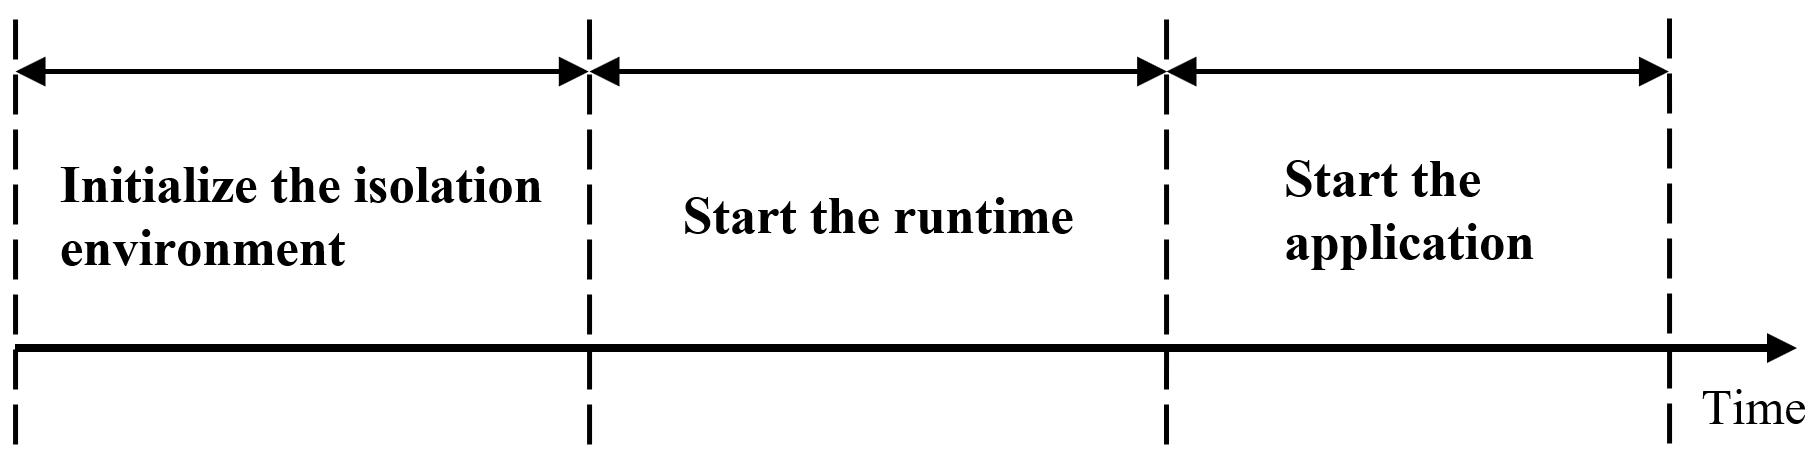
\includegraphics[width=\linewidth]{images/startup-periods.PNG}
    \caption{Startup process of a serverless function}
    \label{startup-periods}
\end{figure}

\subsection{Existing Startup Optimizations}
\label{section:optimization}

\subsubsection{Cache-based Optimizations}
Many systems\cite{pool1,pool2} adopt a pooling strategy to cache function instances.
When request come,
a pre-warmed function instance is taken out from the pool to handle the request,
thereby improving the execution performance of the system.
Although the cache-based strategies can greatly reduce the response latency of serverless computing platforms,
it also reduces the resource utilization of the system and increases costs.
At the same time, it brings great difficulties to the elastic scaling of function instances.

\subsubsection{Isolation Sandbox Optimizations}
By optimizing the isolation sandbox of serverless functions,
the startup performance of the function can be improved.
For example,
FAASM\cite{faasm} introduces the SFI mechanism used in WebAssembly to isolate the memory space of serverless functions.
SFI allows multiple serverless functions to share memory resources while isolating memory.
For the limiting of other resources(such as CPU and network), FAASM uses standard Linux cgroups.
FAASM also provides a low-level POSIX interface for isolated serverless functions to operate on the network and filesystem.
gVisor\cite{gvisor} is a new type of sandbox technology released by Google,
which is essentially a system kernel written in Go language and running in user mode.
Depending on its configuration,
gVisor can use the corresponding mechanism provided by ptrace or KVM to intercept the system calls of the application,
and act as a guest kernel to provide services for the application without using hardware virtualization.
Such a design can bring lower resource consumption,
while reducing the cost of virtualization,
thereby bringing better startup performance.
For most serverless computing applications,
the runtime startup and application startup latency account for a large part. The method of simplifying the isolation environment cannot effectively optimize these stages,
so the overall startup latency is still considerable.

\subsubsection{Checkpoint/Restore-based Optimizations}
SEUSS\cite{seuss}, Catalyz\-er\cite{catalyzer}, Prebaking\cite{prebaking} and other systems use checkpoint technique to create checkpoints on running functions.
By restoring from an existing function checkpoint,
the runtime startup latency and the application startup latency of the function can be effectively reduced.
At the same time,
Catalyzer also optimized the function restore process to further improve the efficiency of function startup.
SEUSS, Catalyzer uses a customized operating system
or modifies the language runtime to achieve the best performance,
but it also brings compatibility issues,
making the system difficult to maintain and manage.
Prebacking restores containerized serverless functions based on the C/S technique provided by CRIU\cite{criu},
but the acceleration mechanism based on restoration still has room for further optimization.
To illustrate this problem,
we use the existing C/S mechanism to restore the function,
as shown in Figure\ref{default-restore} is the restoration latency of some typical serverless functions.

\begin{figure}[t]
    \centering
    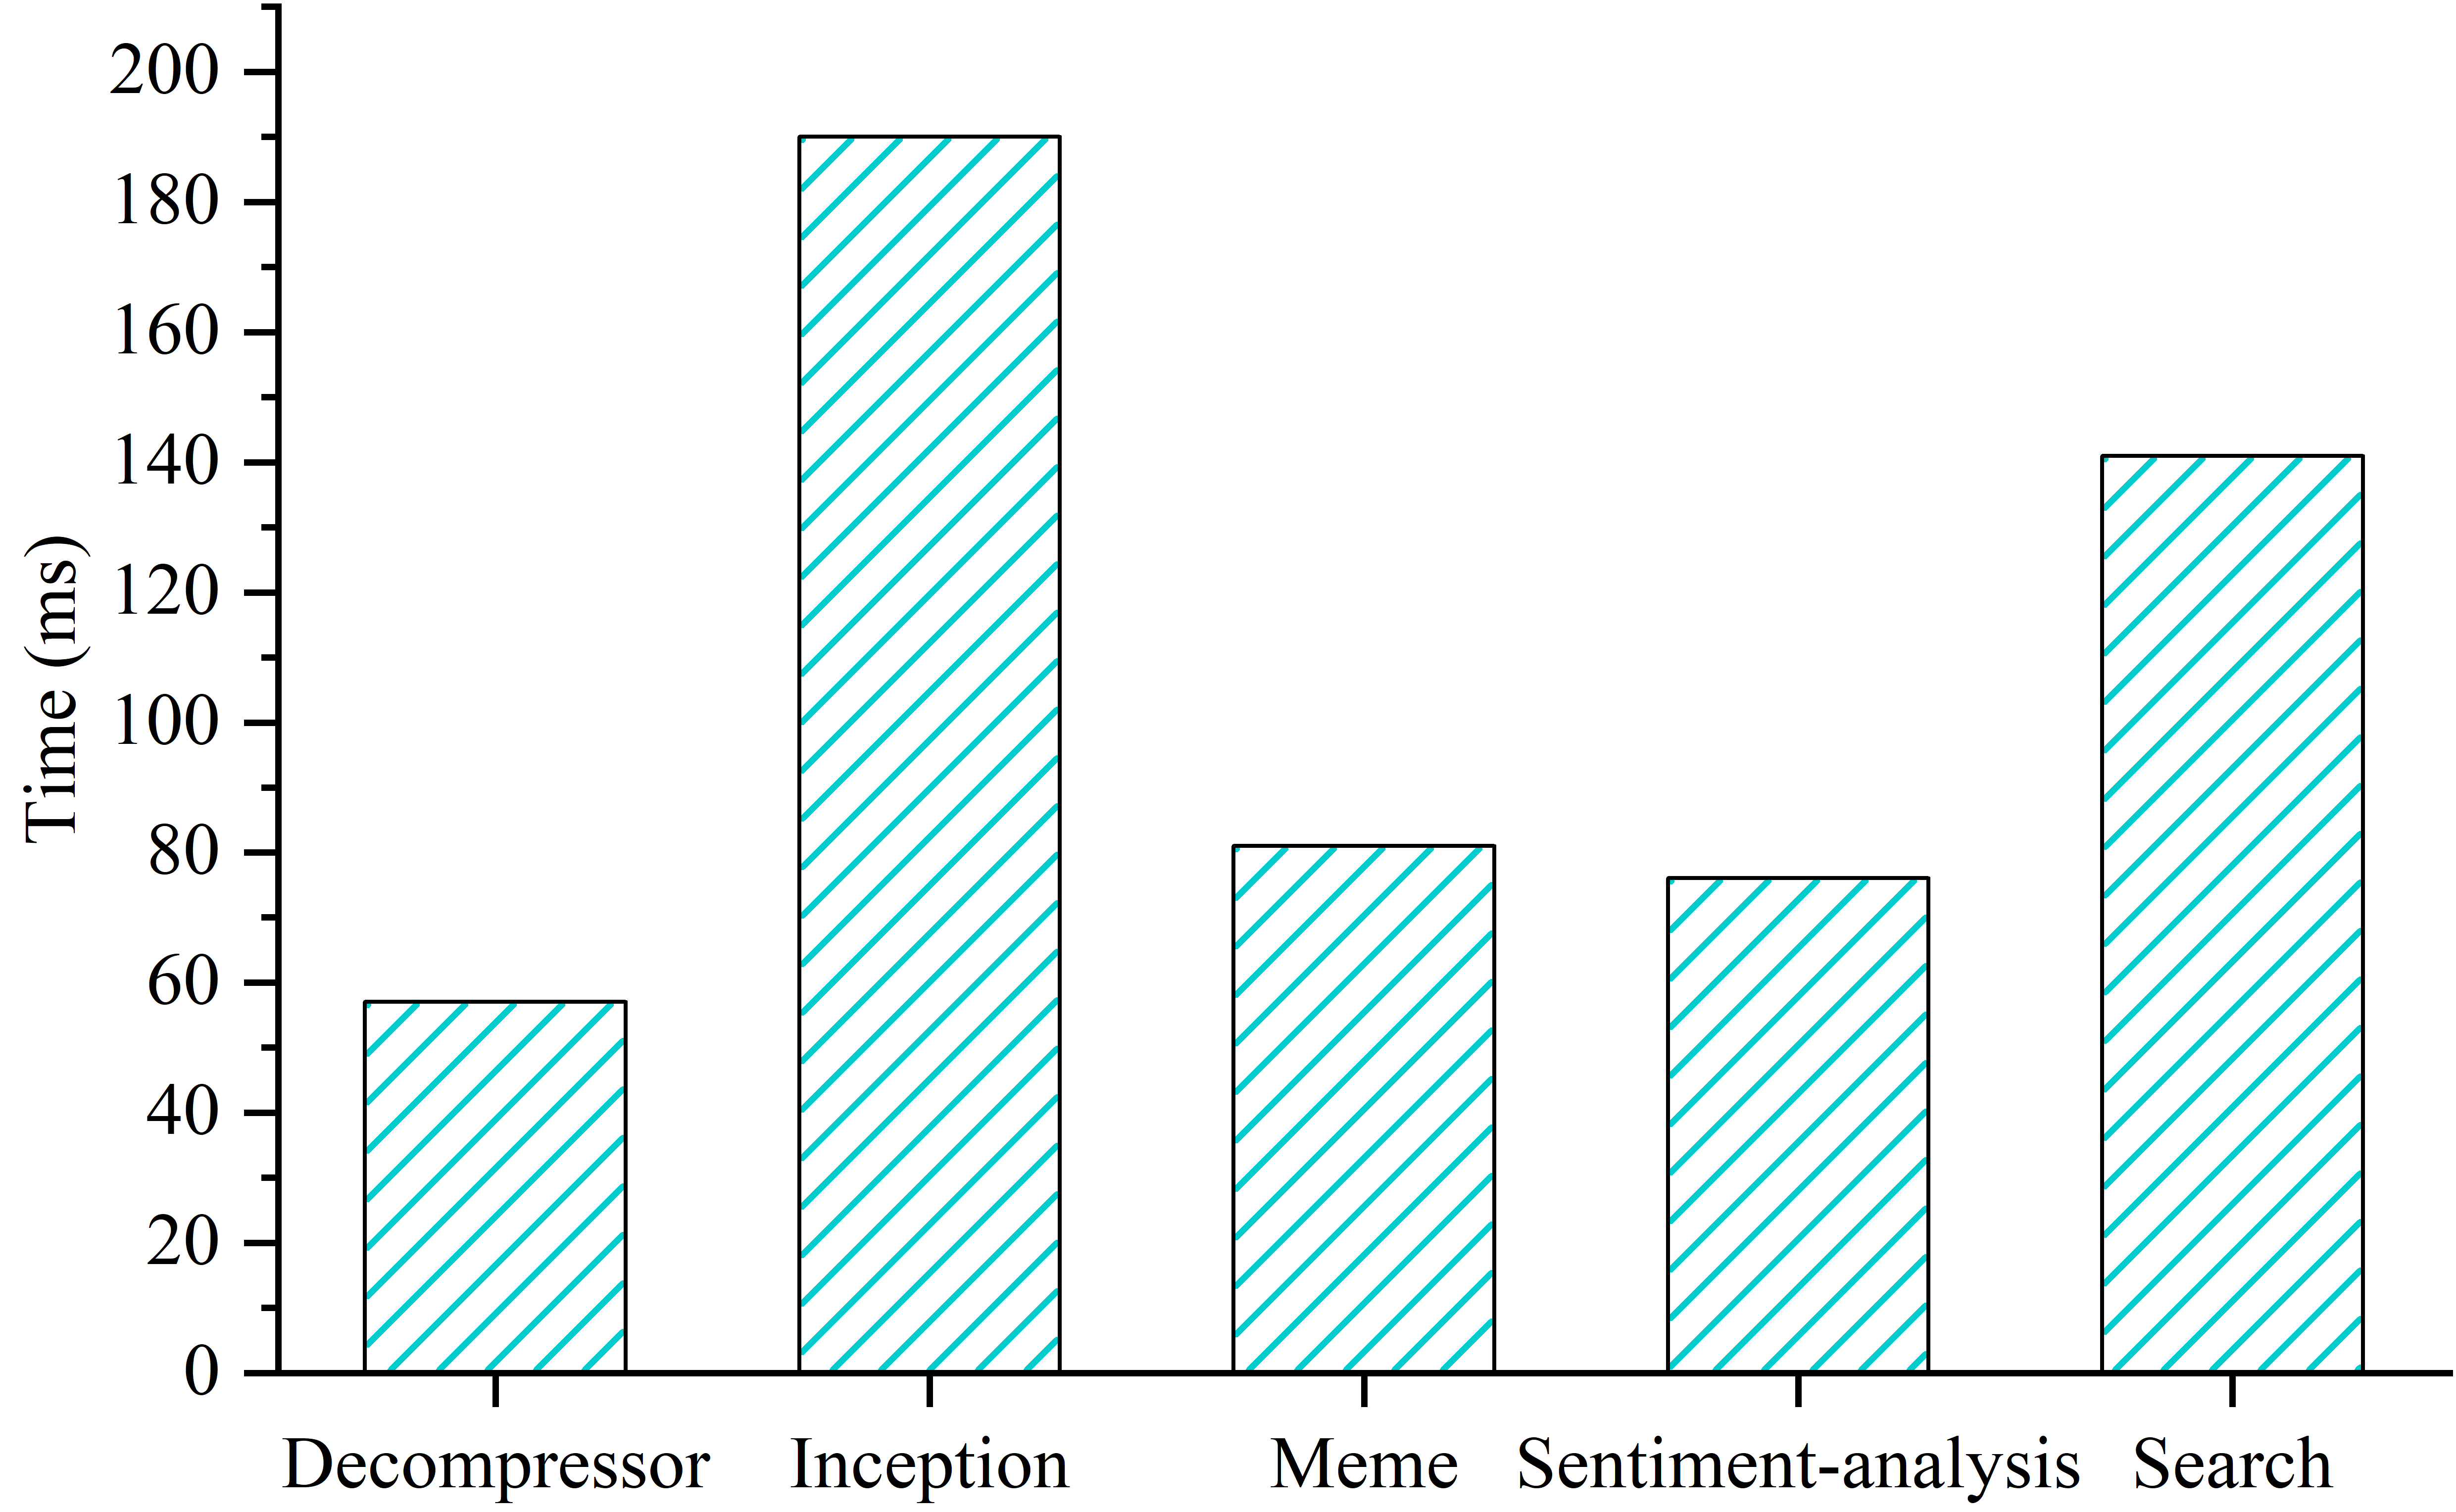
\includegraphics[width=3in]{images/default-restore.png}
    \caption{Restoration latency of serverless functions}
    \label{default-restore}
\end{figure}

Even if the C/S technique is used, some serverless functions still have considerable startup latency,
and the startup latency of functions has great volatility due to the complexity of different applications.
There is another issue worth noting—resource usage.
The figure \ref{restore-mem} is the memory usage of different serverless functions after 10 startups.
Due to the completely independent memory space between each function process,
it causes extreme large resource consumption,
which is not conducive to the large-scale deployment of serverless functions.

\begin{figure}[t]
    \centering
    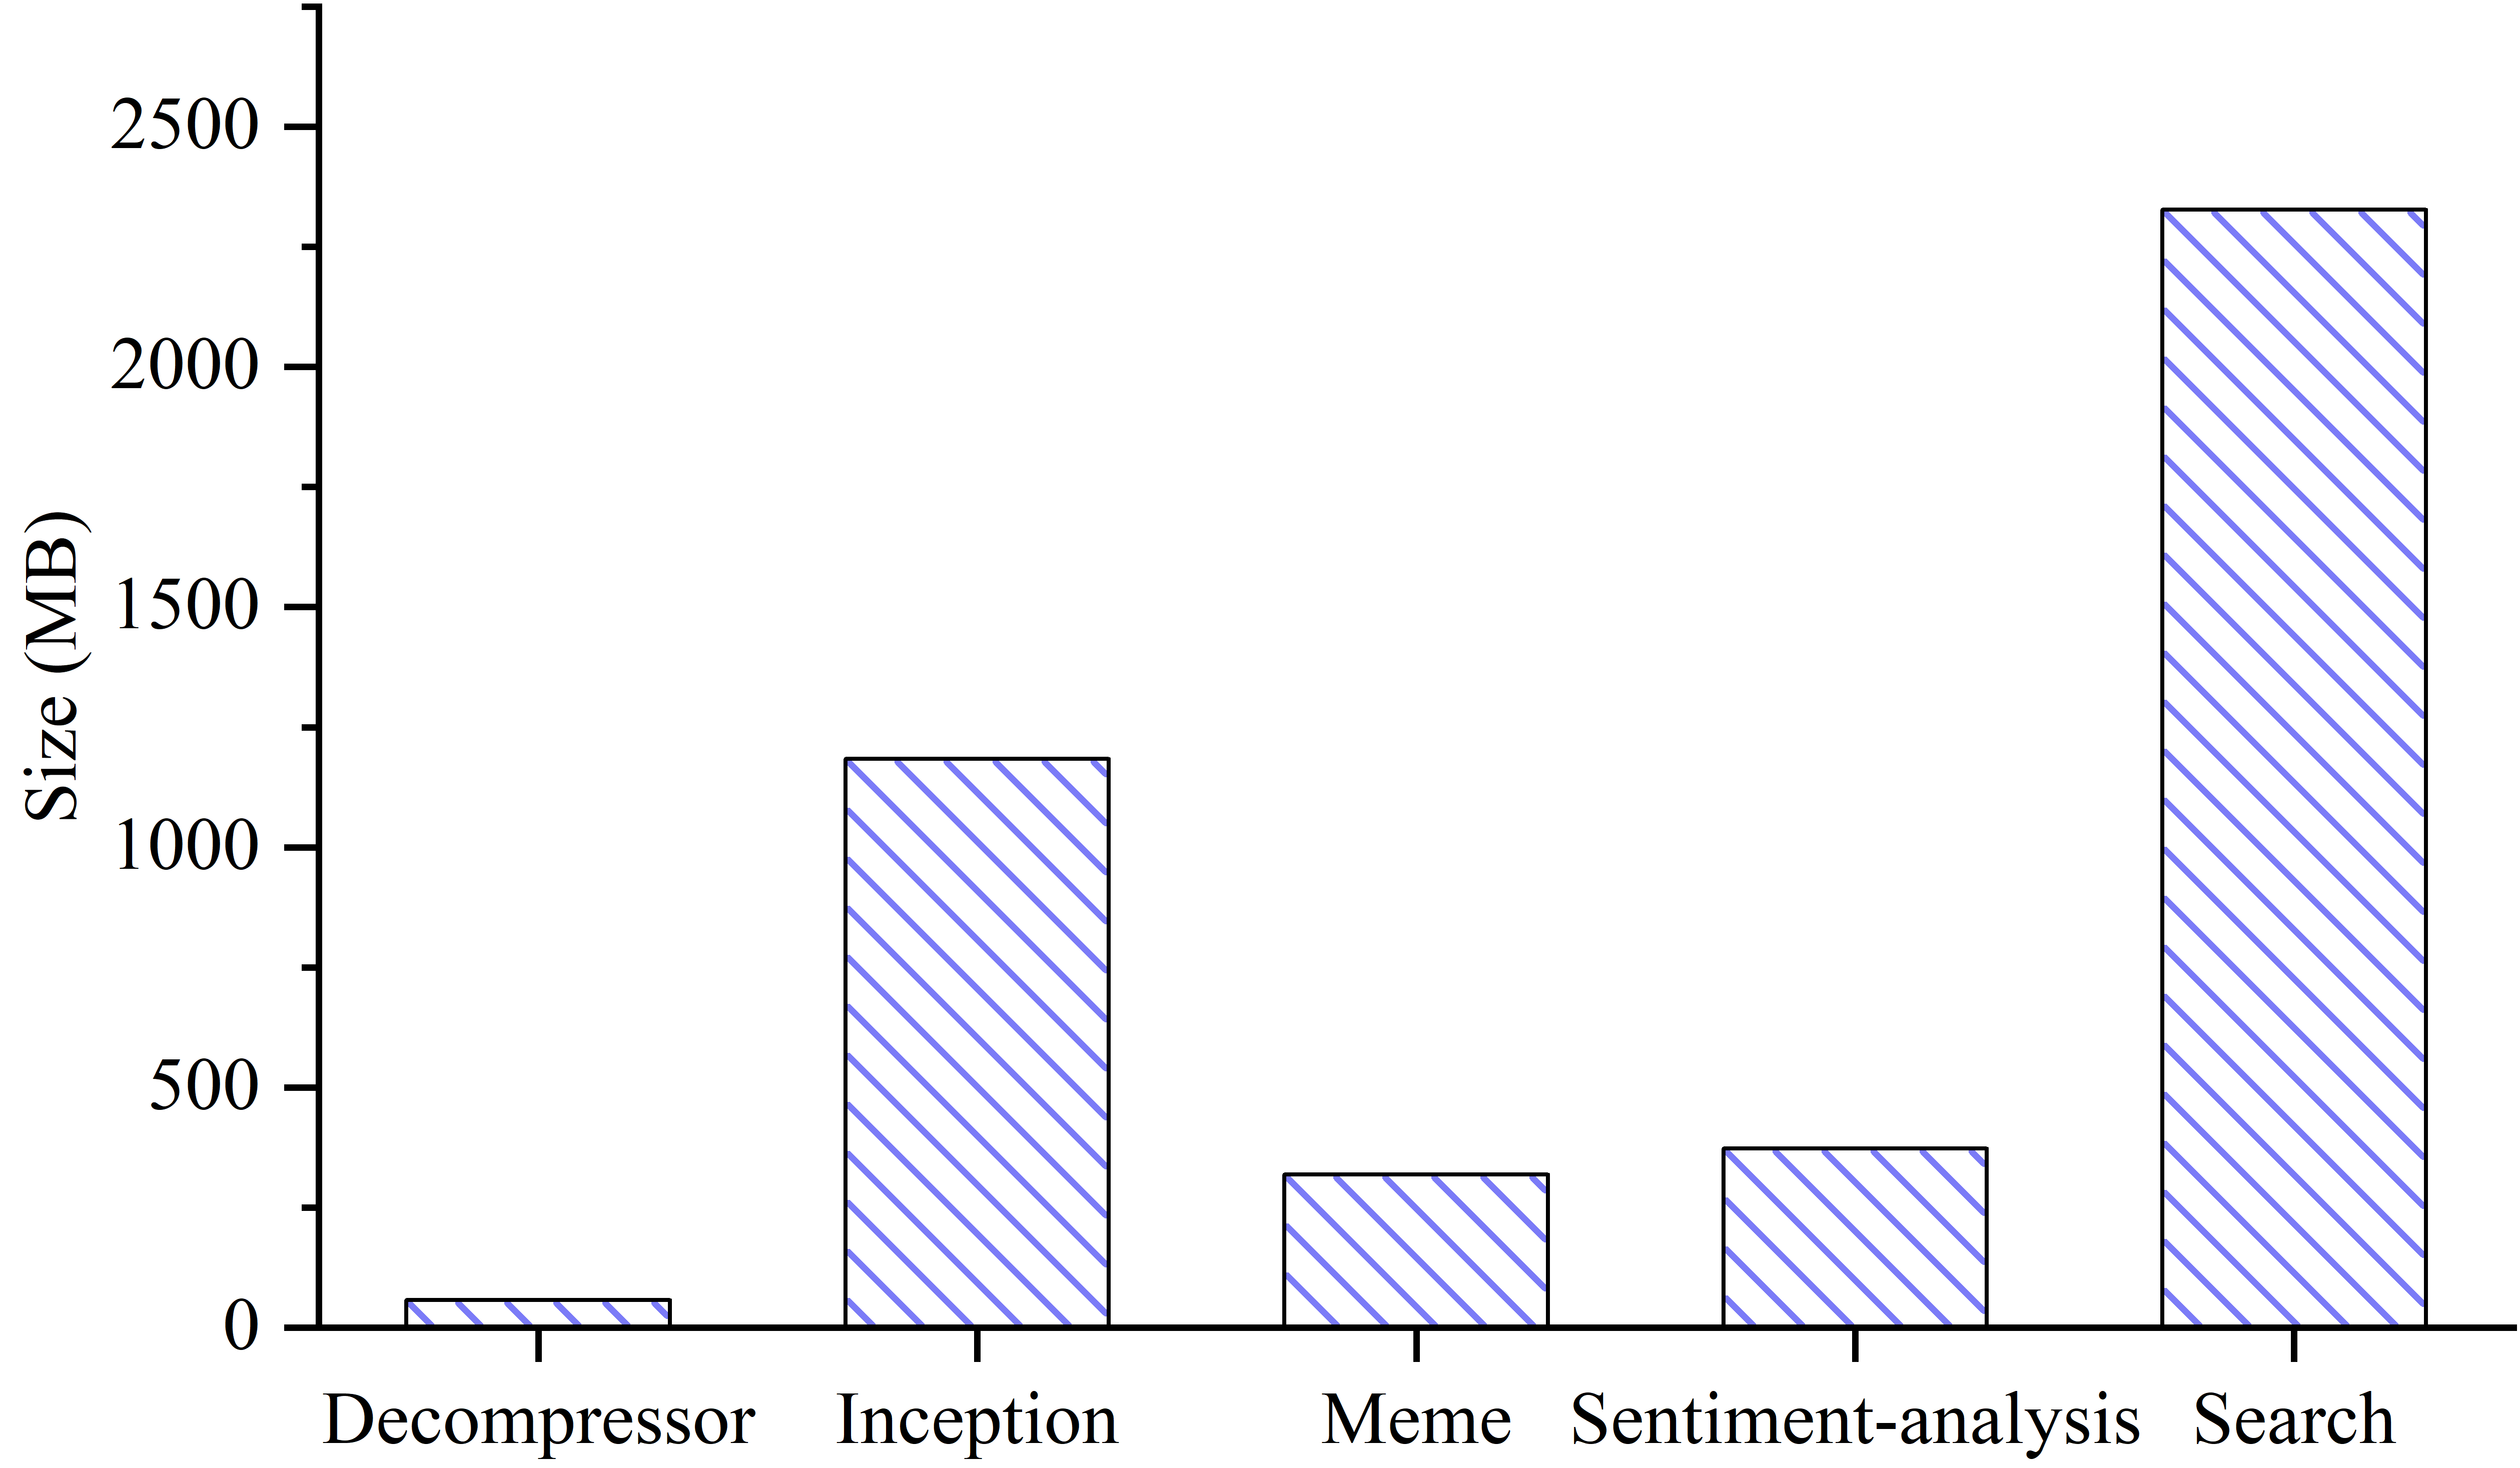
\includegraphics[width=3in]{images/default-resotre-mem.png}
    \caption{Memory usage of serverless functions after 10 starts}
    \label{restore-mem}
\end{figure}

\subsection{Analysis of Serverless Function Restoring Process}


\begin{figure*}[t]
    \centering
    \subfigure[\label{golang-restore}A Golang-based function]{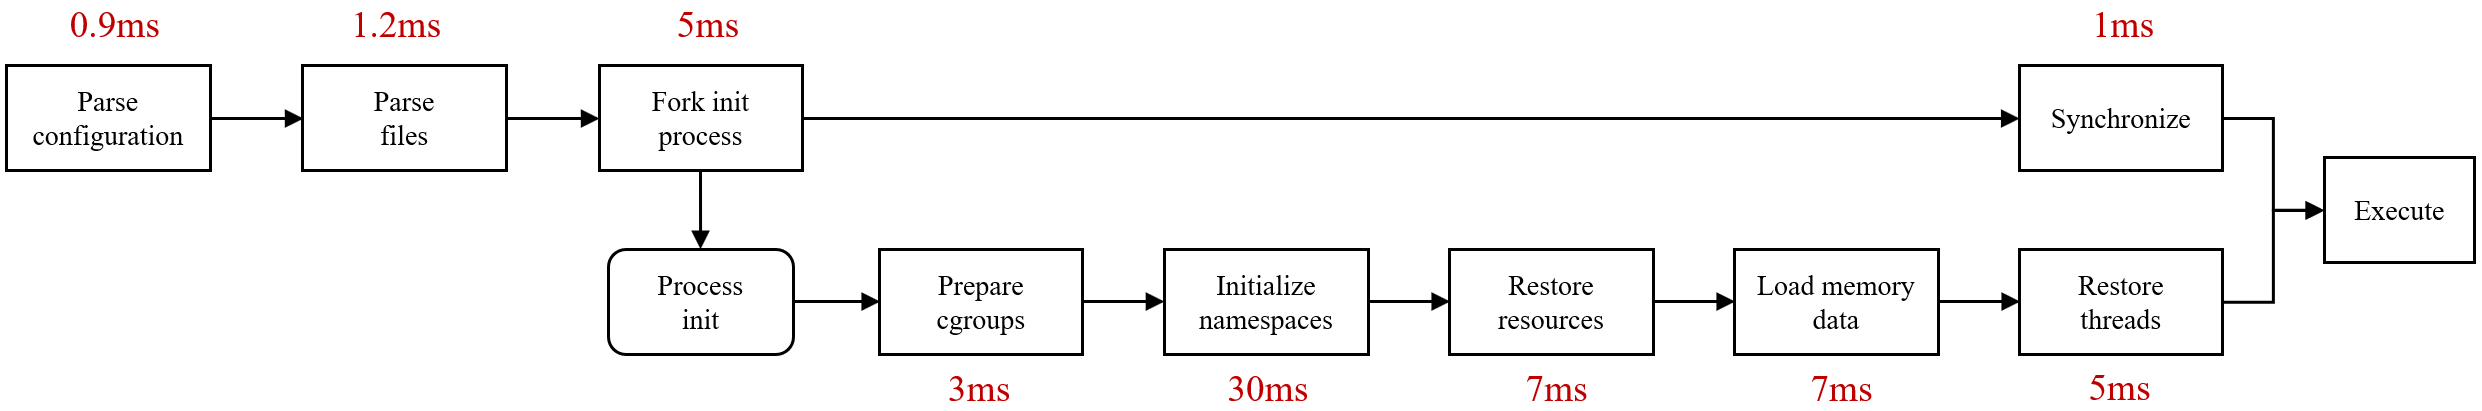
\includegraphics[width=6.5in]{images/golang-restore.PNG}}
    \subfigure[\label{java-restore}A Java-based function]{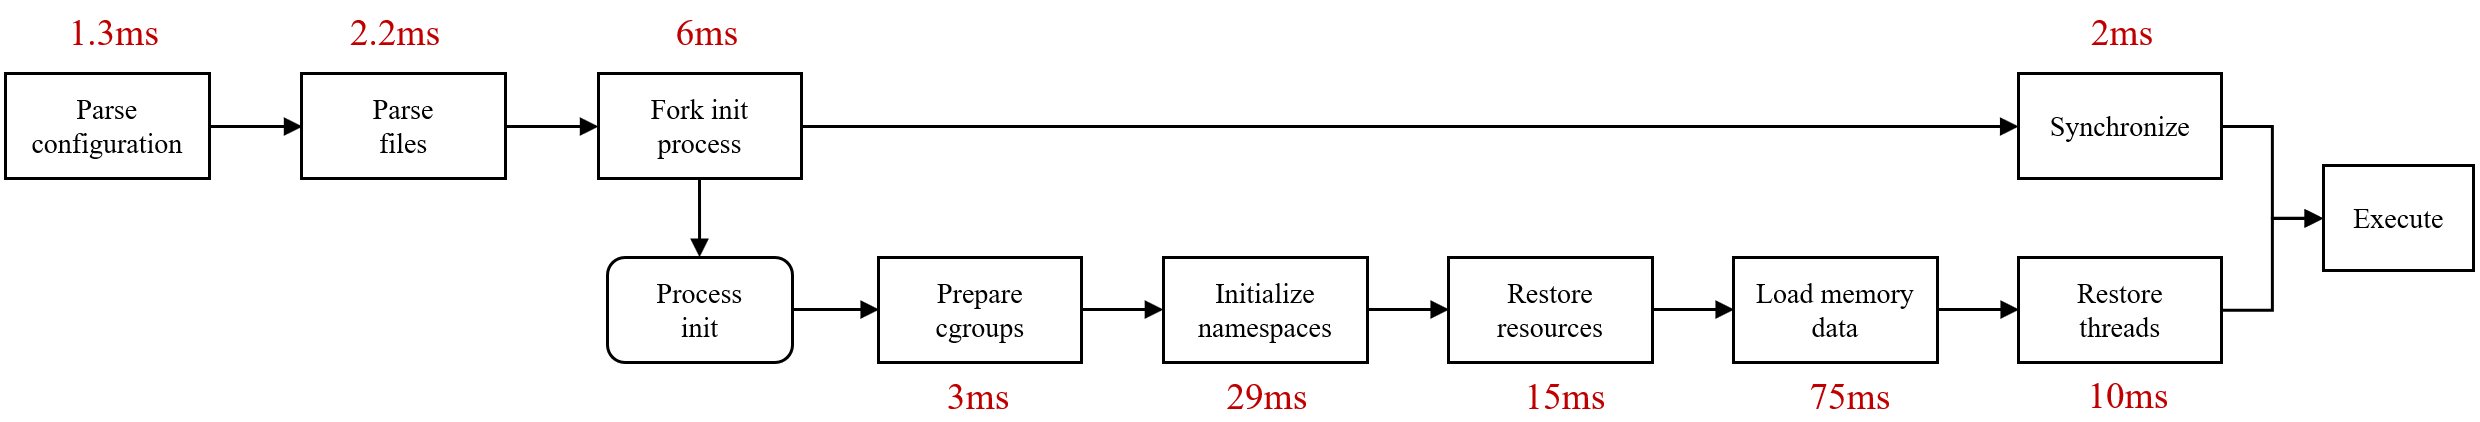
\includegraphics[width=6.5in]{images/java-restore.PNG}}
    \caption{Restoration process of serverless functions}
    \label{restore-process}
\end{figure*}

The containerized serverless function will go through multiple stages as shown in the figure\ref{restore-process} during recovery,
which mainly include configuration analysis,
init process creation,
isolation environment initialization,
resource restoration,
memory data loading,
thread restoration, etc.

In the namespace initialization stage,
CRIU will create multiple brand new namespaces,
and then configure these namespaces according to the contents of the checkpoint.
For example,
for Mount namespace,
CRIU mounts filesystems and devices according to the relevant information from the checkpoint, and for IPC namespace,
CRIU restores Linux system V IPC items.
These additional restoration work brings a fixed and considerable delay to the start of the function.
However, in the memory loading stage,
CRIU copies all memory data to the memory space of the function process,
because different serverless functions have different memory footprints,
the delay in this stage varies.
For example,
Java-based serverless functions(figure \ref{java-restore}) have higher memory loading latency than Golang-based(figure \ref{golang-restore}) functions. 
The way of copying makes multiple function processes have independent memory data, 
resulting in data redundancy.

\textbf{Difficulties in optimization.} Although the initilization of the isolation environment can be optimized by simply simplifying the isolation environment, 
it will reduce the isolation strength and the security of the container. 
At the same time, memory data is necessary for the running of the function, and this stage cannot be optimized by omitting data transmission. 
Therefore, 
the main difficulty lies in how to combine the characteristics of the container environment to speed up the initialization process of the sandbox, 
while adopting an appropriate method to reduce the amount of memory data read during the function startup process, 
improve the initialization efficiency and ensure the correctness of the function.